% !TEX program = xelatex
\documentclass[aspectratio=169]{beamer}

% \usepackage{blindtext}

\usetheme{Execushares}

\graphicspath{{./images/}}

\usepackage{amsmath}

\title{Can statistics help us to understand deep learning?}
\author{Hannes Smit}
\date{2019-03-27}

\setcounter{showSlideNumbers}{1}

\begin{document}
\setcounter{showProgressBar}{0}
\setcounter{showSlideNumbers}{0}

\frame{\titlepage}

\setcounter{framenumber}{0}
\setcounter{showProgressBar}{1}
\setcounter{showSlideNumbers}{1}

\section{Introduction}
\begin{frame}
	\frametitle{Machine Learning}
	\begin{itemize}
		\item Successes
		      \begin{itemize}
			      \item Self driving cars --- safer than human drivers
			      \item Computer vision --- facial recognition
			      \item Writing text
		      \end{itemize}
		\item Possible problems
		      \begin{itemize}
			      \item Self driving cars --- what if they crash?
			      \item Parole decisions in the U.S. --- biases
			      \item GPT2 --- the algorithm `too dangerous to release'
		      \end{itemize}
	\end{itemize}
\end{frame}

\begin{frame}
	\frametitle{The Black Box}
	\begin{itemize}
		\item Machine learning is a black box
		\item We need to be able to open the black box
		\item Put the algorithms' decisions into human understandable terms
	\end{itemize}
\end{frame}

\section{Artificial Neural Networks}
\begin{frame}
	\frametitle{Neuron}
	\begin{columns}
		\column{0.5\textwidth}
		\begin{enumerate}
			\item Weighted sum
			\item Bias term \(b\)
			\item Nonlinear activation function \(\phi\)
			      \begin{itemize}
				      \item Identity (linear regression)
				      \item tanh
				      \item ReLU
			      \end{itemize}
		\end{enumerate}
		\[ y = \phi\left(b + \sum_{i=1}^n w_i x_i\right) \]

		\column{0.5\textwidth}
		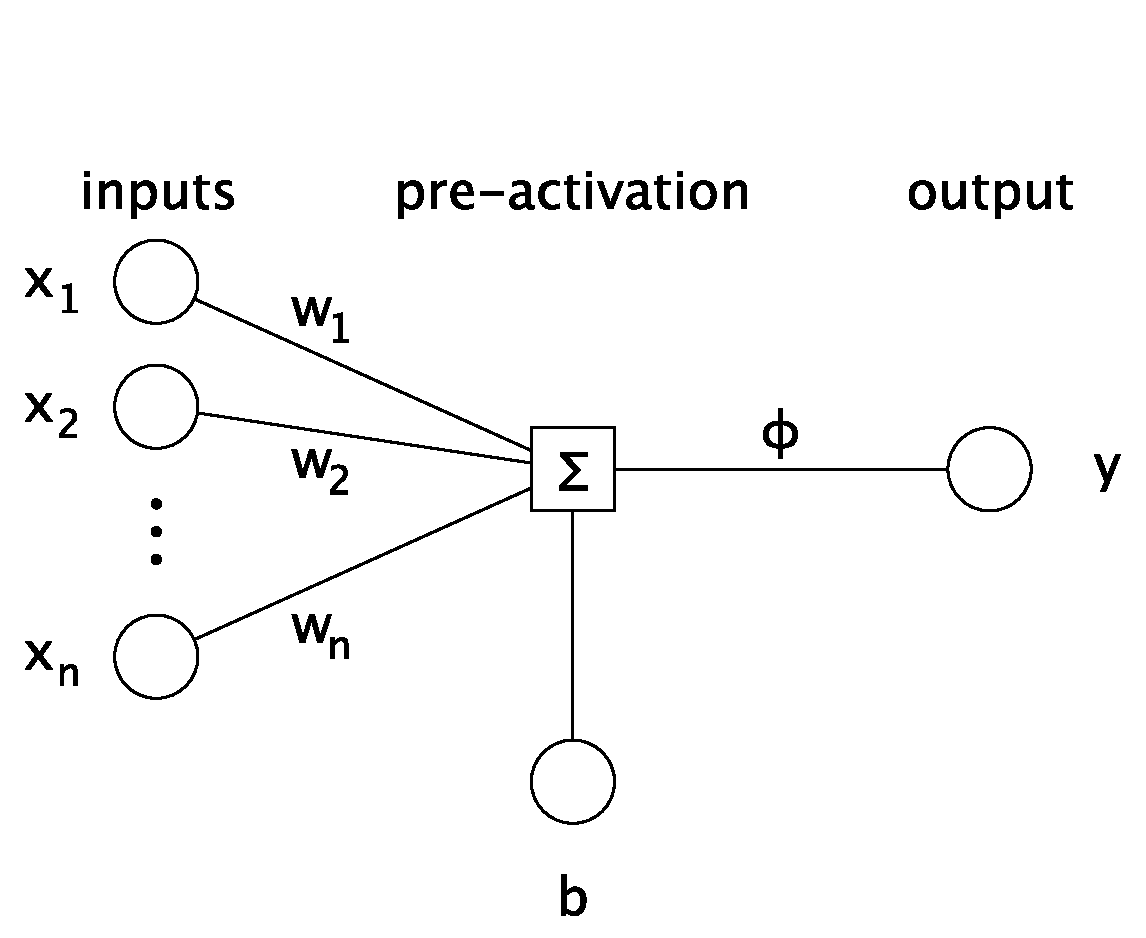
\includegraphics[width=\linewidth]{neuron.pdf}
	\end{columns}
\end{frame}

\begin{frame}
	\frametitle{Backpropogation}
	\begin{figure}
		\centering
		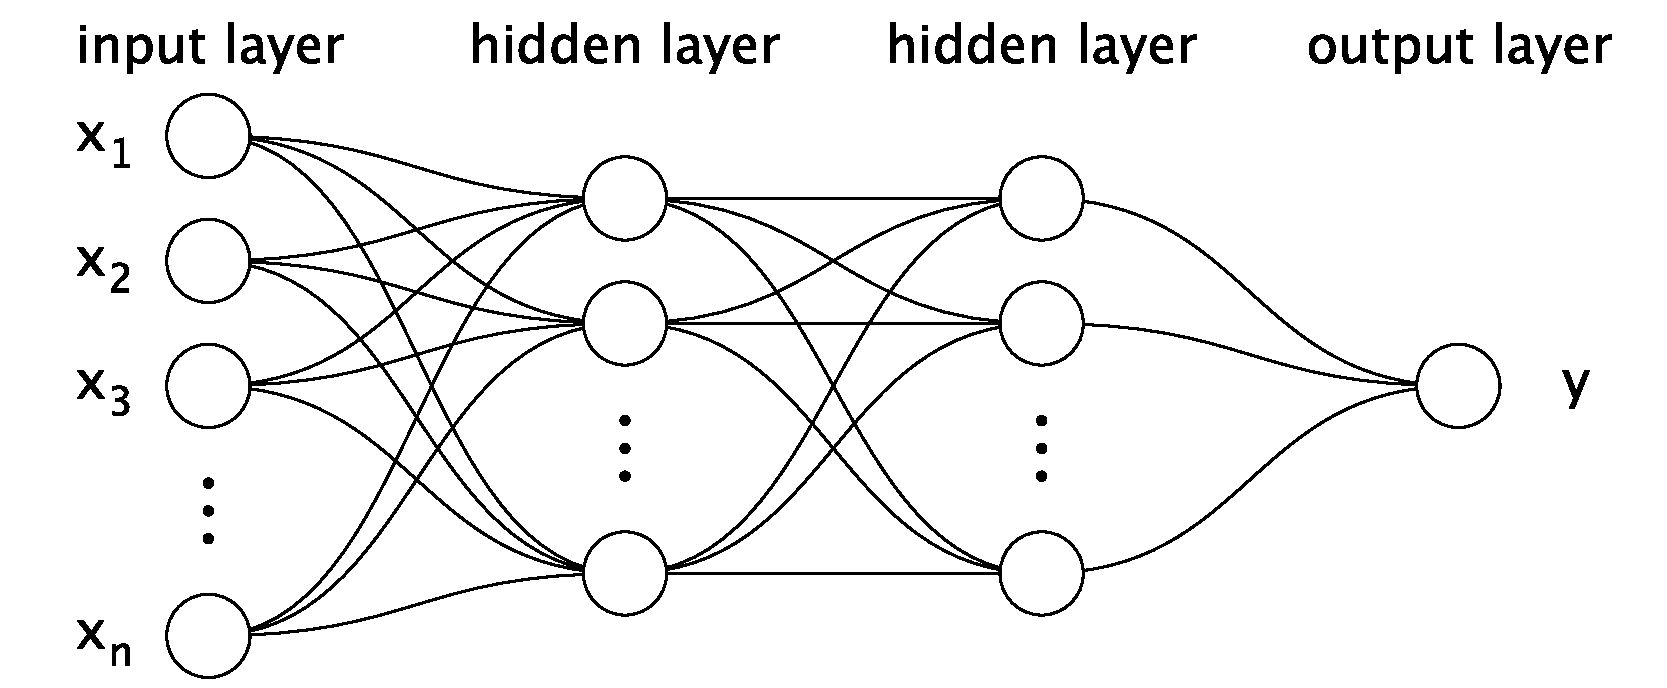
\includegraphics[width=0.7\linewidth]{nn-structure.pdf}
	\end{figure}
	\vspace*{-0.25cm}
	\begin{itemize}
		\item Neural networks are arranged in layers
		\item Deep learning involves many layers
		\item Use gradient descent to optimise the weights
		\item In practice, stochastic batch gradient descent is used
	\end{itemize}
\end{frame}

\begin{frame}
	\frametitle{Simple Example}
	\[ y = x + 5 \sin(x) + \epsilon \quad \epsilon \sim N(0, 0.5) \]
	\begin{figure}
		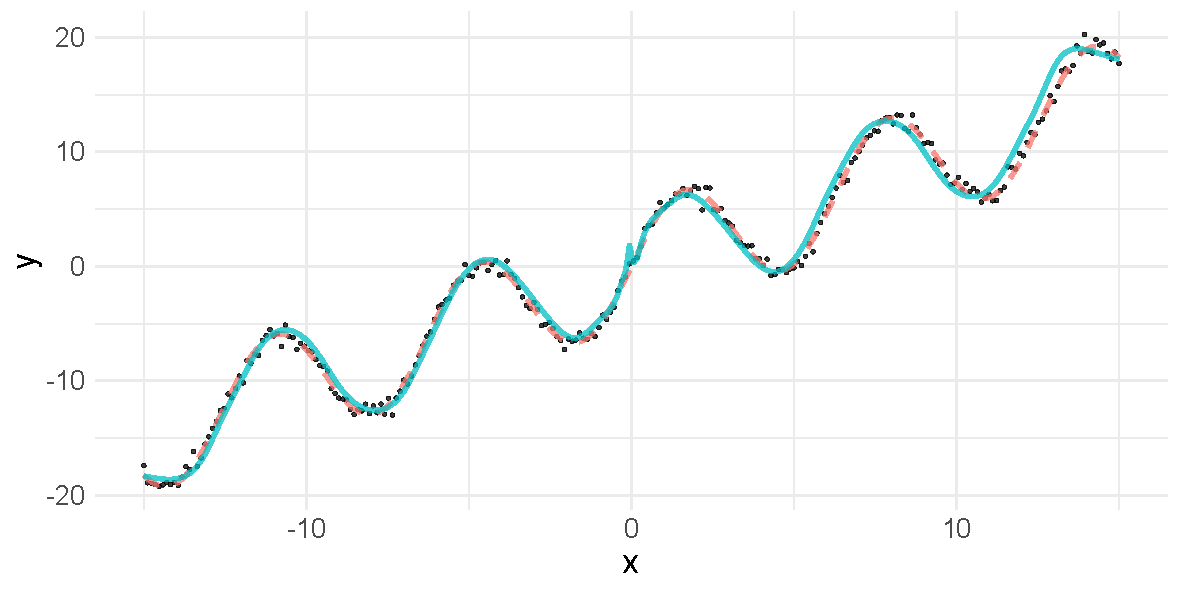
\includegraphics[width=0.8\linewidth]{ann-trained.pdf}
	\end{figure}
\end{frame}

\begin{frame}
	\frametitle{Training}
	\begin{figure}
		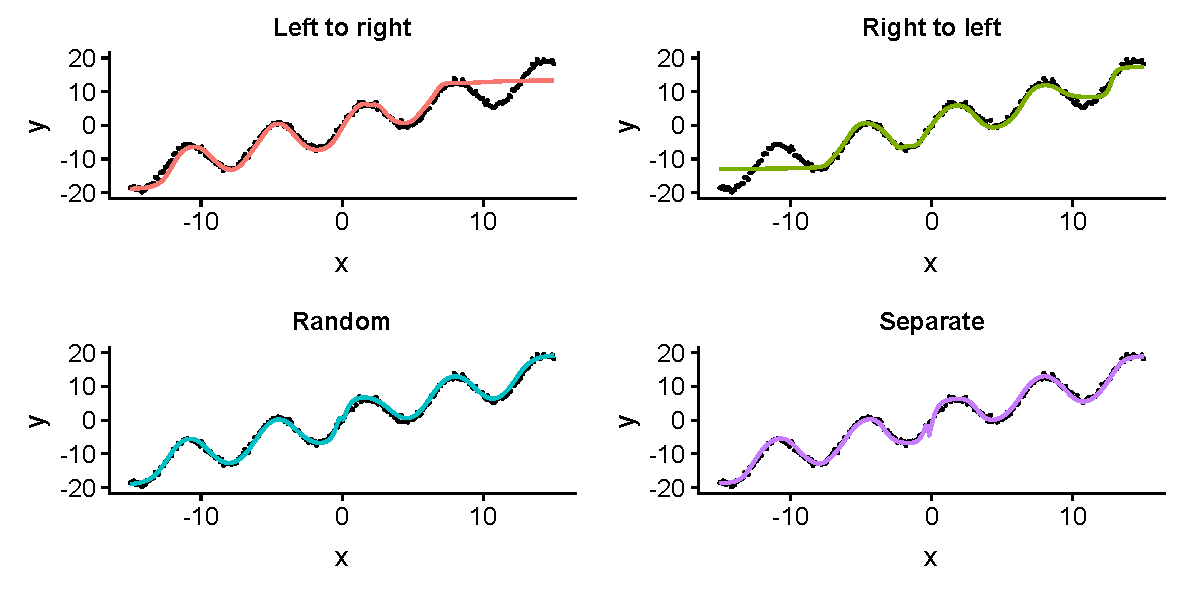
\includegraphics[width=0.9\linewidth]{compare-nn-order.pdf}
	\end{figure}
\end{frame}

\section{Opening the Black Box}
\begin{frame}
	\frametitle{Current Research}

\end{frame}

\begin{frame}
	\frametitle{Linear Regression}
	\[ y = x + 5 \sin(x) + \epsilon \quad \epsilon \sim N(0, 0.5) \]
	\begin{align*}
		y = & \alpha + \beta_0 x + \beta_1 x^2 +                                \\
		    & \beta_2 \sin(x) + \beta_3 \sin(2x) + \beta_4 \sin(x/2) +          \\
		    & \beta_5 \cos(x) + \beta_6 \cos(2x) + \beta_7 \cos(x/2) + \epsilon
	\end{align*}
\end{frame}

\begin{frame}
	\frametitle{Linear Regression Results}
	\[ y = x + 5 \sin(x) + \epsilon \quad \epsilon \sim N(0, 0.5) \]
	\begin{table}
		\centering
		\begin{tabular}{rrrrrl}
			\hline
			              & Estimate & Std. Error & t value & p value &                \\
			\hline
			(Intercept)   & 0.1404   & 0.0695     & 2.02    & 0.0444  &                \\
			\(x\)         & 1.0203   & 0.0053     & 193.86  & 0.0000  & \(\leftarrow\) \\
			\(x^2\)       & 0.0006   & 0.0007     & 0.87    & 0.3843  &                \\
			\(\sin(x)\)   & 4.7783   & 0.0643     & 74.31   & 0.0000  & \(\leftarrow\) \\
			\(\sin(2x)\)  & 0.0720   & 0.0636     & 1.13    & 0.2588  &                \\
			\(\sin(x/2)\) & 0.0099   & 0.0662     & 0.15    & 0.8808  &                \\
			\(\cos(x)\)   & 0.2785   & 0.0656     & 4.25    & 0.0000  & \(\leftarrow\) \\
			\(\cos(2x)\)  & 0.0654   & 0.0647     & 1.01    & 0.3130  &                \\
			\(\cos(x/2)\) & 0.0901   & 0.0705     & 1.28    & 0.2028  &                \\
			\hline
		\end{tabular}
	\end{table}
\end{frame}

\begin{frame}
	\frametitle{Stepwise Regression}
	\begin{table}
		\centering
		\begin{tabular}{rrrrr}
			\hline
			             & Estimate & Std. Error & t value & p value \\
			\hline
			(Intercept)  & 0.1840   & 0.0458     & 4.02    & 0.0001         \\
			\(x\)        & 1.0201   & 0.0052     & 195.05  & 0.0000         \\
			\(sin(x)\)   & 4.7815   & 0.0633     & 75.54   & 0.0000         \\
			\(cos(x)\)   & 0.2864   & 0.0652     & 4.40    & 0.0000         \\
			\(cos(x/2)\) & 0.1146   & 0.0637     & 1.80    & 0.0732         \\
			\hline
		\end{tabular}
	\end{table}
\end{frame}

\begin{frame}
	\frametitle{Stepwise Regression}
	\begin{figure}
		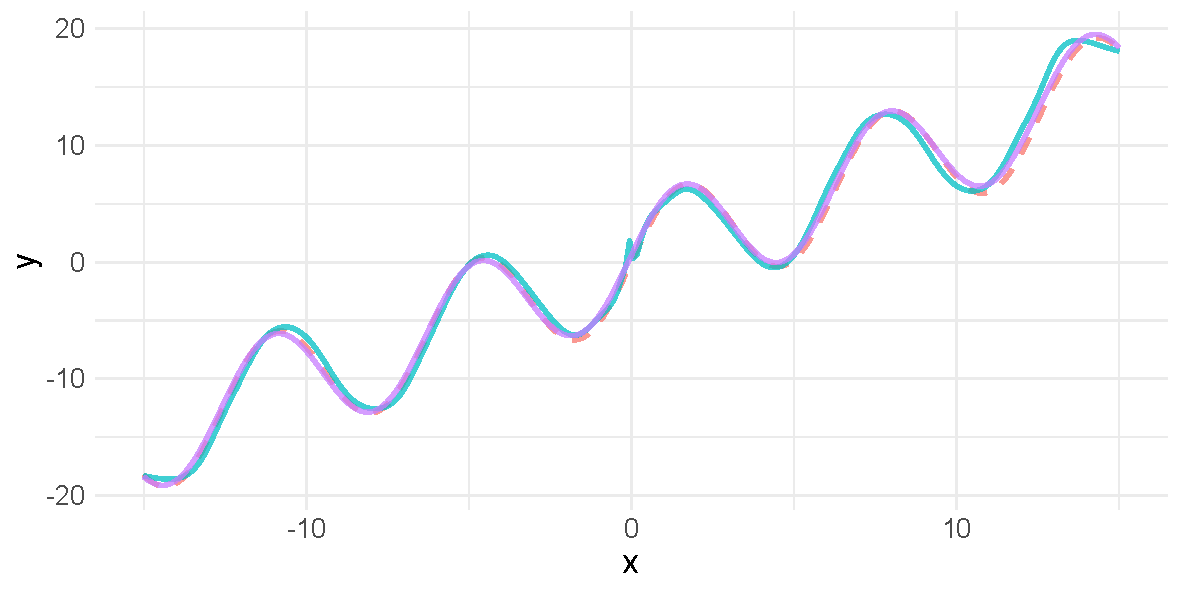
\includegraphics[width=0.9\linewidth]{stepwise-fit.pdf}
	\end{figure}
\end{frame}

\begin{frame}
	\frametitle{Lasso}
	\begin{columns}
		\column{0.5\textwidth}
		\begin{itemize}
			\item Least Absolute Shrinkage and Selection Operator
			\item Constrains the sum of the absolute values of the model parameters
			\item Regularises the least influential parameters to zero
			\item Use k-fold cross validation to find the optimal hyperparameter \(\lambda\)
		\end{itemize}
		\column{0.5\textwidth}
		\begin{figure}
			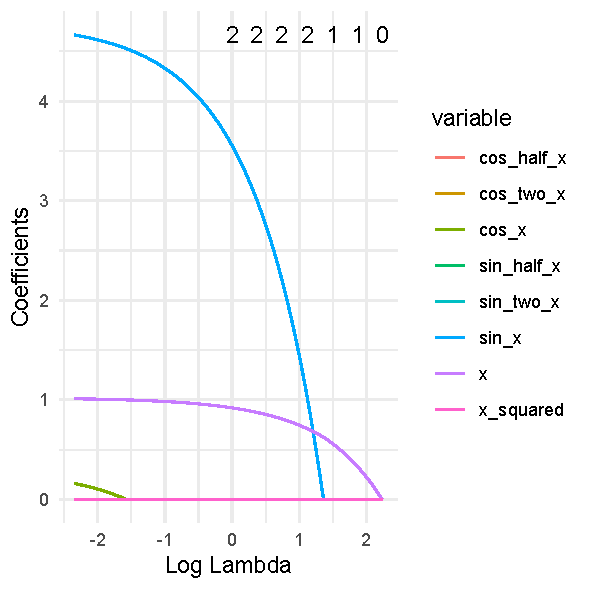
\includegraphics[width=\linewidth]{lasso-lambda.pdf}
		\end{figure}
	\end{columns}

\end{frame}

\begin{frame}
	\frametitle{Lasso Results}
	\begin{columns}
		\column{0.5\textwidth}
		Result of 10 fold CV: \(\lambda = -2.232497\)
		\begin{table}[ht]
			\centering
			\begin{tabular}{rr}
				\hline
				variable    & estimate \\
				\hline
				(Intercept) & 0.20     \\
				\(x\)       & 1.01     \\
				\(\sin(x)\) & 4.64     \\
				\(\cos(x)\) & 0.13     \\
				\hline
			\end{tabular}
		\end{table}
		\column{0.5\textwidth}
		\begin{figure}
			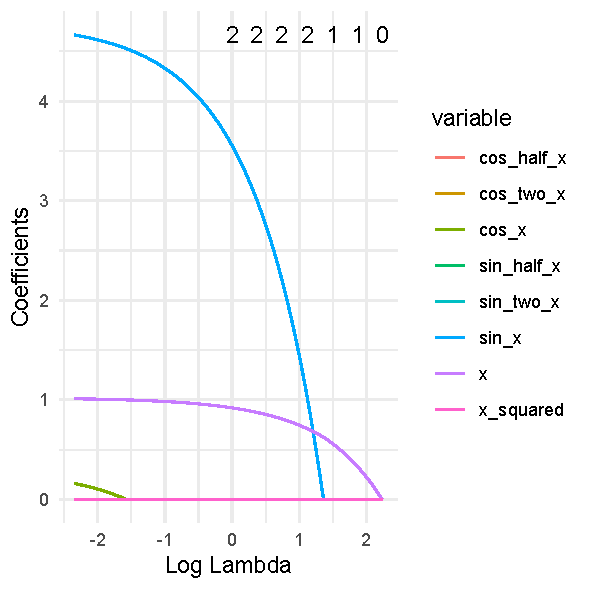
\includegraphics[width=\linewidth]{lasso-lambda.pdf}
		\end{figure}
	\end{columns}
\end{frame}

\begin{frame}
	\frametitle{Gaussian Processes}
	\begin{itemize}
		\item A Gaussian Process is the infinite dimensional analogue to the multivariate normal distribution
		\item Instead of a mean vector it uses a mean function and instead of a covariance matrix it uses a covariance function
		\item GPs have statistical properties that are understood
	\end{itemize}
\end{frame}

\begin{frame}
	\frametitle{Using a Gaussian Process}
	\begin{figure}
		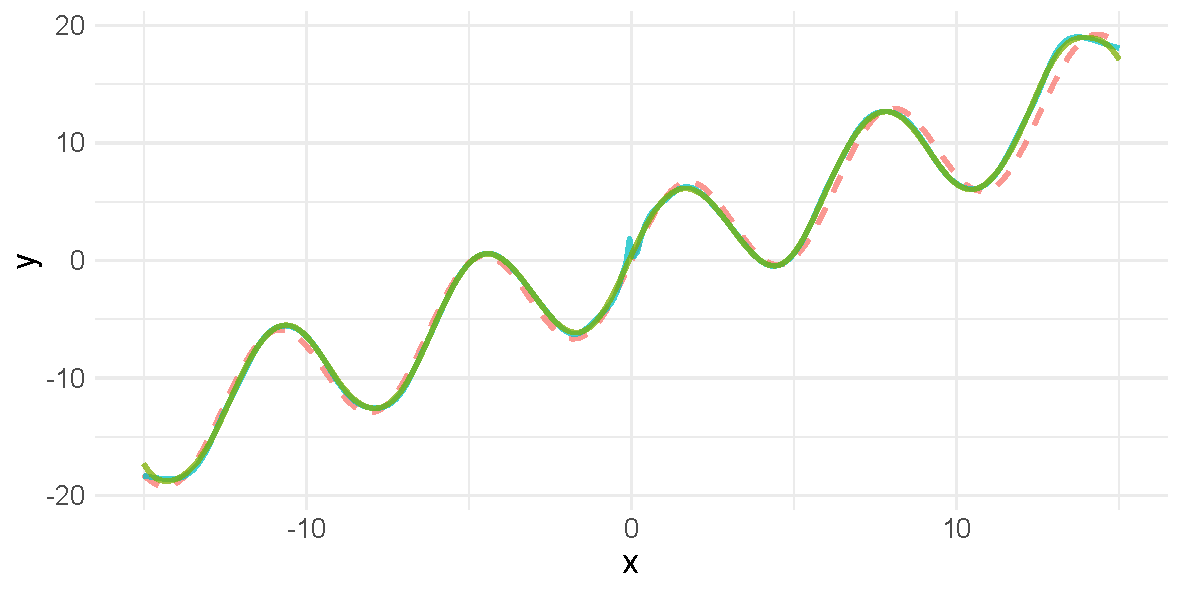
\includegraphics[width=0.9\linewidth]{gp-trained.pdf}
	\end{figure}
\end{frame}

\begin{frame}
	\frametitle{Future Research}
	\begin{itemize}
		\item Using these techniques on more complex and realistic problems
		\item Use the Lasso method as a mean function for a Gaussian process
		\item Sensitivity analysis can also find significant variables
	\end{itemize}
\end{frame}
\section{Thank you for listening}
\end{document}
